% Options for packages loaded elsewhere
\PassOptionsToPackage{unicode}{hyperref}
\PassOptionsToPackage{hyphens}{url}
%
\documentclass[
  12pt,
  a4paper,
  DIV=11,
  numbers=noendperiod]{scrreprt}

\usepackage{amsmath,amssymb}
\usepackage{setspace}
\usepackage{iftex}
\ifPDFTeX
  \usepackage[T1]{fontenc}
  \usepackage[utf8]{inputenc}
  \usepackage{textcomp} % provide euro and other symbols
\else % if luatex or xetex
  \usepackage{unicode-math}
  \defaultfontfeatures{Scale=MatchLowercase}
  \defaultfontfeatures[\rmfamily]{Ligatures=TeX,Scale=1}
\fi
\usepackage{lmodern}
\ifPDFTeX\else  
    % xetex/luatex font selection
\fi
% Use upquote if available, for straight quotes in verbatim environments
\IfFileExists{upquote.sty}{\usepackage{upquote}}{}
\IfFileExists{microtype.sty}{% use microtype if available
  \usepackage[]{microtype}
  \UseMicrotypeSet[protrusion]{basicmath} % disable protrusion for tt fonts
}{}
\usepackage{xcolor}
\setlength{\emergencystretch}{3em} % prevent overfull lines
\setcounter{secnumdepth}{5}
% Make \paragraph and \subparagraph free-standing
\ifx\paragraph\undefined\else
  \let\oldparagraph\paragraph
  \renewcommand{\paragraph}[1]{\oldparagraph{#1}\mbox{}}
\fi
\ifx\subparagraph\undefined\else
  \let\oldsubparagraph\subparagraph
  \renewcommand{\subparagraph}[1]{\oldsubparagraph{#1}\mbox{}}
\fi


\providecommand{\tightlist}{%
  \setlength{\itemsep}{0pt}\setlength{\parskip}{0pt}}\usepackage{longtable,booktabs,array}
\usepackage{calc} % for calculating minipage widths
% Correct order of tables after \paragraph or \subparagraph
\usepackage{etoolbox}
\makeatletter
\patchcmd\longtable{\par}{\if@noskipsec\mbox{}\fi\par}{}{}
\makeatother
% Allow footnotes in longtable head/foot
\IfFileExists{footnotehyper.sty}{\usepackage{footnotehyper}}{\usepackage{footnote}}
\makesavenoteenv{longtable}
\usepackage{graphicx}
\makeatletter
\def\maxwidth{\ifdim\Gin@nat@width>\linewidth\linewidth\else\Gin@nat@width\fi}
\def\maxheight{\ifdim\Gin@nat@height>\textheight\textheight\else\Gin@nat@height\fi}
\makeatother
% Scale images if necessary, so that they will not overflow the page
% margins by default, and it is still possible to overwrite the defaults
% using explicit options in \includegraphics[width, height, ...]{}
\setkeys{Gin}{width=\maxwidth,height=\maxheight,keepaspectratio}
% Set default figure placement to htbp
\makeatletter
\def\fps@figure{htbp}
\makeatother

\KOMAoption{captions}{tableheading}
\usepackage{indentfirst}
\usepackage{float}
\floatplacement{figure}{H}
\usepackage[math,RM={Scale=0.94},SS={Scale=0.94},SScon={Scale=0.94},TT={Scale=MatchLowercase,FakeStretch=0.9},DefaultFeatures={Ligatures=Common}]{plex-otf}
\makeatletter
\@ifpackageloaded{caption}{}{\usepackage{caption}}
\AtBeginDocument{%
\ifdefined\contentsname
  \renewcommand*\contentsname{Содержание}
\else
  \newcommand\contentsname{Содержание}
\fi
\ifdefined\listfigurename
  \renewcommand*\listfigurename{Список иллюстраций}
\else
  \newcommand\listfigurename{Список иллюстраций}
\fi
\ifdefined\listtablename
  \renewcommand*\listtablename{Список таблиц}
\else
  \newcommand\listtablename{Список таблиц}
\fi
\ifdefined\figurename
  \renewcommand*\figurename{Рисунок}
\else
  \newcommand\figurename{Рисунок}
\fi
\ifdefined\tablename
  \renewcommand*\tablename{Таблица}
\else
  \newcommand\tablename{Таблица}
\fi
}
\@ifpackageloaded{float}{}{\usepackage{float}}
\floatstyle{ruled}
\@ifundefined{c@chapter}{\newfloat{codelisting}{h}{lop}}{\newfloat{codelisting}{h}{lop}[chapter]}
\floatname{codelisting}{Список}
\newcommand*\listoflistings{\listof{codelisting}{Листинги}}
\makeatother
\makeatletter
\makeatother
\makeatletter
\@ifpackageloaded{caption}{}{\usepackage{caption}}
\@ifpackageloaded{subcaption}{}{\usepackage{subcaption}}
\makeatother
\ifLuaTeX
\usepackage[bidi=basic]{babel}
\else
\usepackage[bidi=default]{babel}
\fi
\babelprovide[main,import]{russian}
\babelprovide[import]{english}
% get rid of language-specific shorthands (see #6817):
\let\LanguageShortHands\languageshorthands
\def\languageshorthands#1{}
\ifLuaTeX
  \usepackage{selnolig}  % disable illegal ligatures
\fi
\usepackage[style=gost-numeric,backend=biber,langhook=extras,autolang=other*]{biblatex}
\addbibresource{bib/cite.bib}
\usepackage{csquotes}
\usepackage{bookmark}

\IfFileExists{xurl.sty}{\usepackage{xurl}}{} % add URL line breaks if available
\urlstyle{same} % disable monospaced font for URLs
\hypersetup{
  pdftitle={Отчёт по лабораторной работе №1},
  pdfauthor={Кривобоков Юрий Дмитриевич},
  pdflang={ru-RU},
  hidelinks,
  pdfcreator={LaTeX via pandoc}}

\title{Отчёт по лабораторной работе №1}
\usepackage{etoolbox}
\makeatletter
\providecommand{\subtitle}[1]{% add subtitle to \maketitle
  \apptocmd{\@title}{\par {\large #1 \par}}{}{}
}
\makeatother
\subtitle{Простейший вариант}
\author{Кривобоков Юрий Дмитриевич}
\date{}

\begin{document}
\maketitle

\renewcommand*\contentsname{Содержание}
{
\setcounter{tocdepth}{1}
\tableofcontents
}
\listoffigures
\listoftables
\setstretch{1.5}
\chapter{Цель
работы}\label{ux446ux435ux43bux44c-ux440ux430ux431ux43eux442ux44b}

Целью данной работы является приобретение практических навыков установки
операционной системы на виртуальную машину, настройки минимально
необходимых для дальнейшей работы сервисов.

\chapter{Задание}\label{ux437ux430ux434ux430ux43dux438ux435}

\begin{itemize}
\tightlist
\item
  Установка Linux на VirtualBox
\item
  Установка необходимого ПО
\item
  Первоначальная настройка ОС для дальнейшей работы
\end{itemize}

\chapter{Теоретическое
введение}\label{ux442ux435ux43eux440ux435ux442ux438ux447ux435ux441ux43aux43eux435-ux432ux432ux435ux434ux435ux43dux438ux435}

VirtualBox (Oracle VM VirtualBox) --- программный продукт виртуализации,
который позволяет запускать несколько гостевых операционных систем на
одном компьютере под управлением основной (хостовой) системы.

\chapter{Выполнение лабораторной
работы}\label{ux432ux44bux43fux43eux43bux43dux435ux43dux438ux435-ux43bux430ux431ux43eux440ux430ux442ux43eux440ux43dux43eux439-ux440ux430ux431ux43eux442ux44b}

Создаю виртальный жесткий диск и запускаю скачанный образ операционной
системы. (рис. -\textcite{fig:001})

\begin{figure}

{\centering 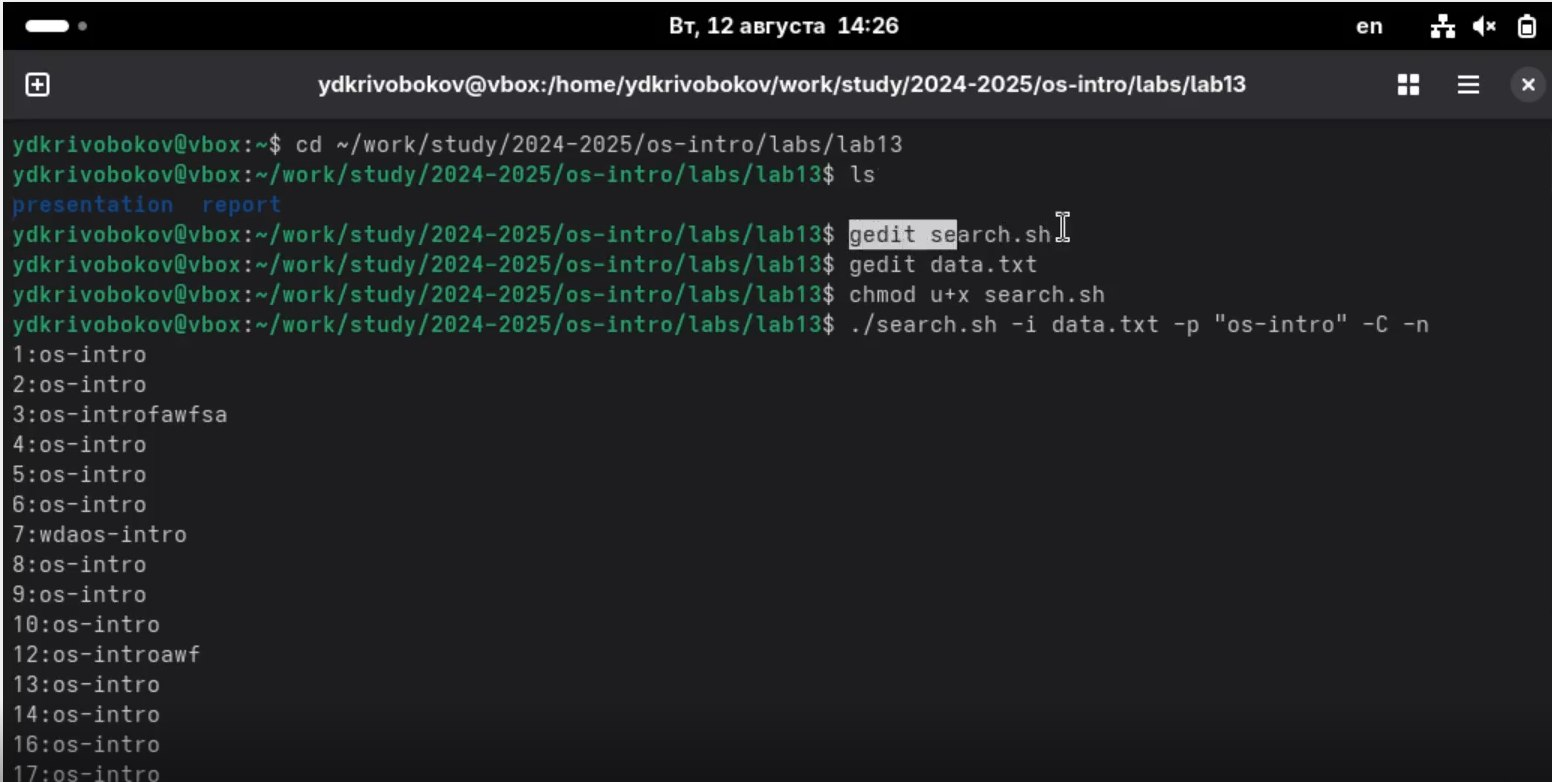
\includegraphics[width=0.7\textwidth,height=\textheight]{image/1.png}

}

\caption{Пример конфигурации QEMU}

\end{figure}%

Через интерактивный установщик задаю базовые настройки для установки
операционной системы. (рис. -\textcite{fig:002})

\begin{figure}

{\centering 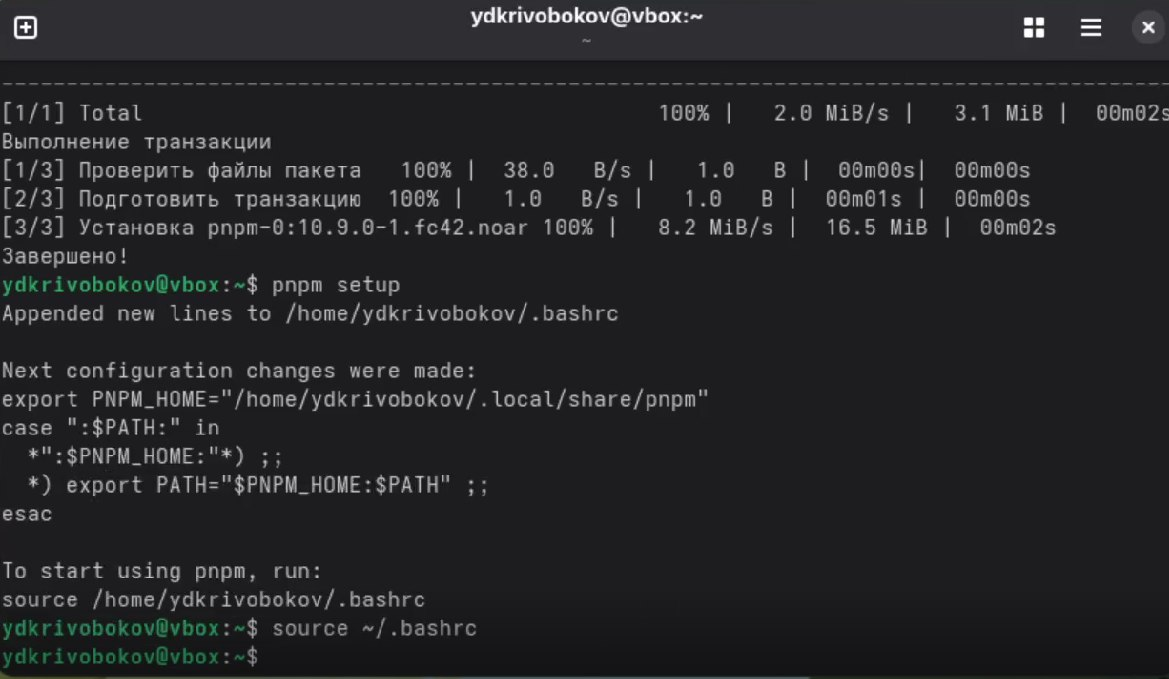
\includegraphics[width=0.7\textwidth,height=\textheight]{image/2.png}

}

\caption{Процесс установки ОС}

\end{figure}%

Продолжаю установку через интерактивный интерфейс. (рис.
-\textcite{fig:003})

\begin{figure}

{\centering 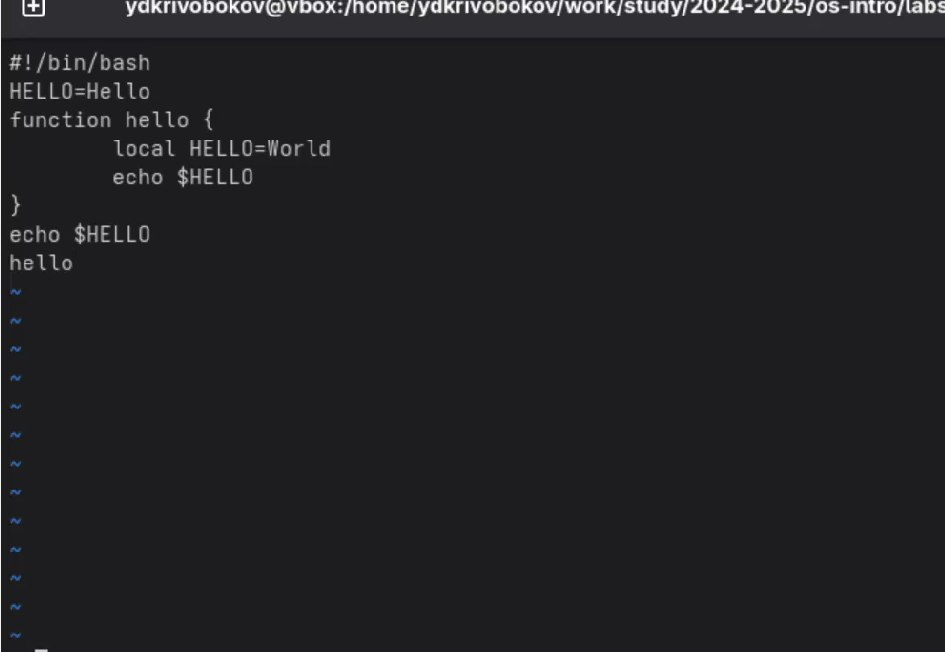
\includegraphics[width=0.7\textwidth,height=\textheight]{image/3.png}

}

\caption{Пример bash скрипта}

\end{figure}%

Скачиваю набор необходимых пакетов для работы с ОС. (рис.
-\textcite{fig:004})

\begin{figure}

{\centering 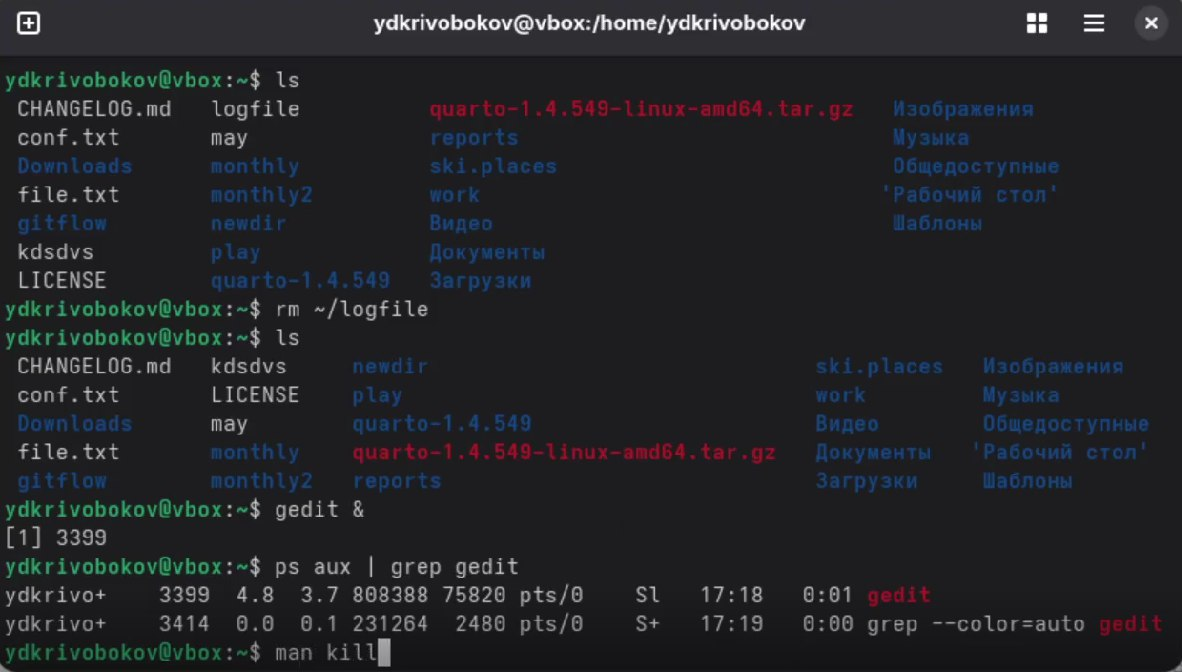
\includegraphics[width=0.7\textwidth,height=\textheight]{image/4.png}

}

\caption{Установка ПО}

\end{figure}%

Продолжаю установку пакетов. (рис. -\textcite{fig:005})

\begin{figure}

{\centering 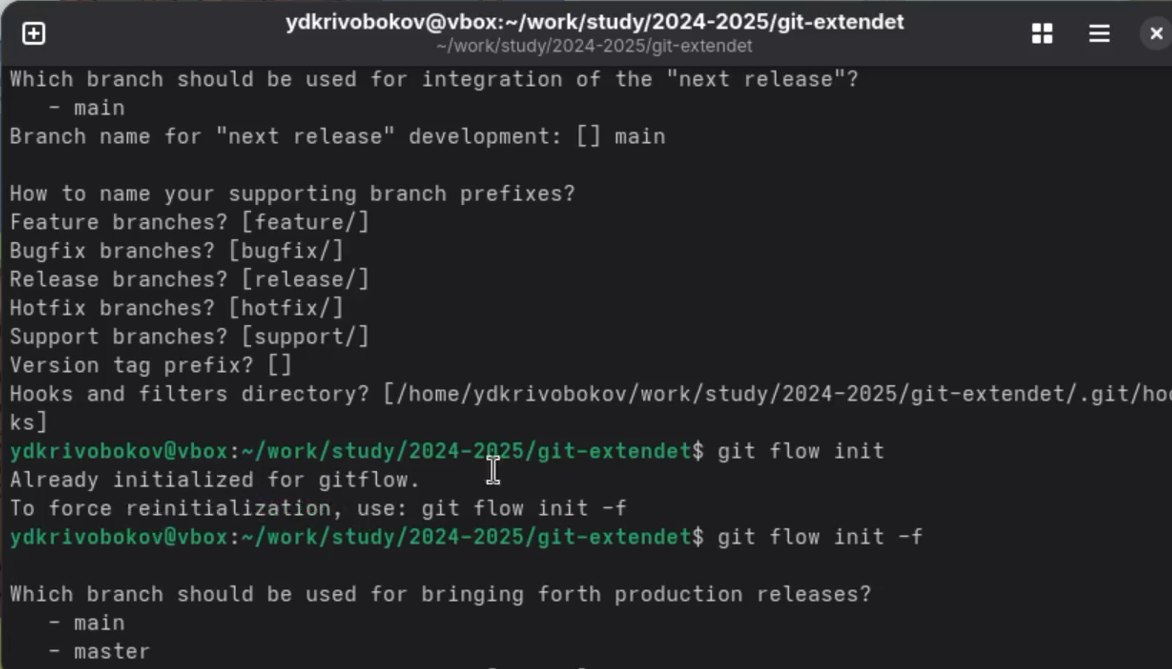
\includegraphics[width=0.7\textwidth,height=\textheight]{image/5.png}

}

\caption{Запуск скрипта}

\end{figure}%

Скачиваю необходимые ресурсы для работы Пандок. (рис.
-\textcite{fig:006})

\begin{figure}

{\centering 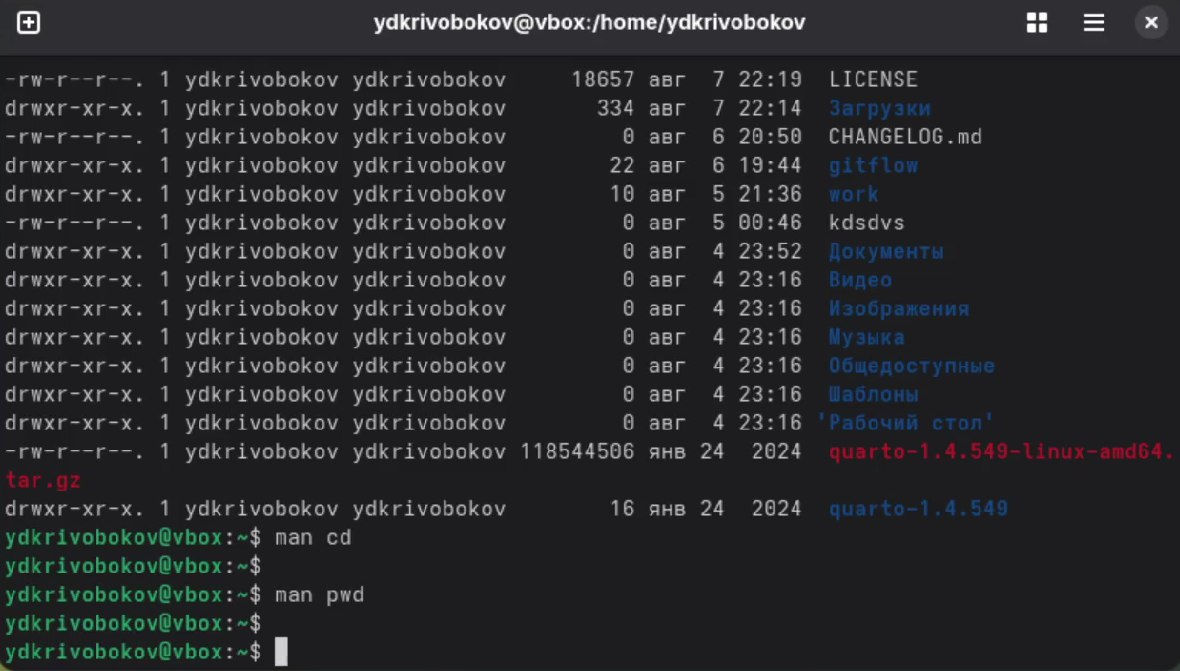
\includegraphics[width=0.7\textwidth,height=\textheight]{image/6.png}

}

\caption{Отключение защиты Linux}

\end{figure}%

\chapter{Домашнее
задание}\label{ux434ux43eux43cux430ux448ux43dux435ux435-ux437ux430ux434ux430ux43dux438ux435}

Проверяю последовательность загрузки графического окружения командой
dmesg \textbar{} grep -i с указанием вывода желаемого нахождения (рис.
-\textcite{fig:010})

\begin{figure}

{\centering 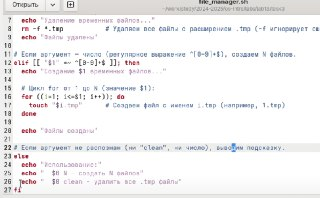
\includegraphics[width=0.7\textwidth,height=\textheight]{image/10.png}

}

\caption{Вывод команды dmesg}

\end{figure}%

\chapter{Выводы}\label{ux432ux44bux432ux43eux434ux44b}

В ходе выполнения лабораторный работы приборел навыки установки
виртуальной машины на Qemu, установил ряд пакетов и настроил ОС для
дальнейшей работы на ней.

\chapter*{Список
литературы}\label{ux441ux43fux438ux441ux43eux43a-ux43bux438ux442ux435ux440ux430ux442ux443ux440ux44b}
\addcontentsline{toc}{chapter}{Список литературы}

\printbibliography[heading=none]




\end{document}
